%  !TeX  root  =  user_guide.tex 

\chapter{Other core plugins}

% when the revision of a section has been finalized, 
% comment out the following line:
% \updatedisclaimer

The remaining core plugins are listed in Table \ref{tab:other_core}, along with references to 
the chapters in this manual which cover their usage.

\begin{table}[H]
\centering
 \begin{tabular}{|l|l|p{8cm}|}
\hline \textbf{Icon} & \textbf{Plugin} & \textbf{Manual Reference}\\
\hline

\includegraphics[width=0.6cm]{diagram_overlay}
 & Diagram Overlay \index{plugins!diagram}& Chapter \ref{sec:diagram}\\
\hline

\includegraphics[width=0.6cm]{grass}
 & GRASS \index{plugin!grass toolbox} & Chapter \ref{sec:grass} and Appendix \ref{appdx_grass_toolbox_modules}\\
 \hline
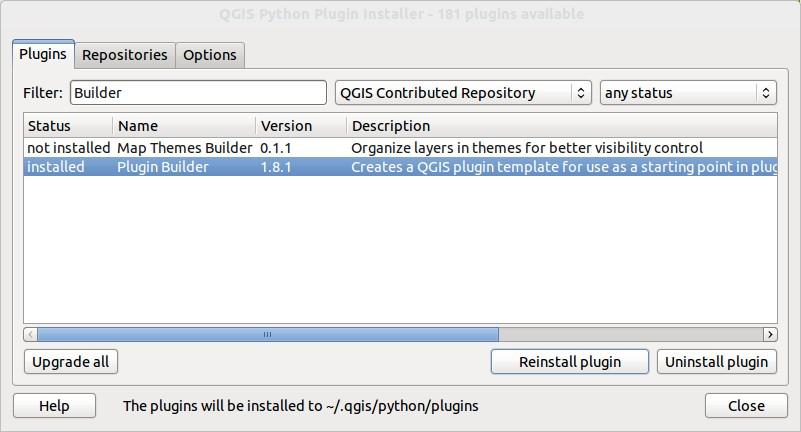
\includegraphics[width=0.6cm]{plugin_installer}
 & Plugin Installer \index{plugins!Plugin Installer} & Chapter \ref{sec:python_plugin_installer}\\
\hline

\includegraphics[width=0.6cm]{spiticon}
 & SPIT \index{plugins!spit}& Chapter \ref{sec:loading_postgis_data} \\
 \hline

\includegraphics[width=0.6cm]{mIconAddWfsLayer}
 & WFS & Chapter \ref{sec:ogc-wfs} \\
\hline
\end{tabular}
\caption{Other Core Plugins}\label{tab:other_core}
\end{table}
